\documentclass[12pt,a4paper]{article}

\usepackage[utf8]{inputenc}
\usepackage[T1]{fontenc}

\usepackage{geometry}
\usepackage{amsmath,amssymb}
\usepackage{booktabs}
\usepackage{array}
\usepackage{listings}
\usepackage{xcolor}
\usepackage{hyperref}
\usepackage{fancyhdr}
\usepackage{parskip}
\usepackage{enumitem}
\usepackage{float}
\usepackage{tikz}
\usetikzlibrary{positioning}

\geometry{margin=2.5cm}

\definecolor{codegray}{rgb}{0.95,0.95,0.95}
\definecolor{codeblue}{rgb}{0.13,0.29,0.53}

\lstdefinestyle{pseudo}{
  backgroundcolor=\color{blue!5},
  basicstyle=\ttfamily\small,
  breaklines=true,
  frame=single,
  rulecolor=\color{blue!30},
  numbers=left,
  numberstyle=\tiny\color{gray},
  numbersep=8pt,
  tabsize=2,
  showstringspaces=false,
  captionpos=b,
}

\pagestyle{fancy}
\fancyhf{}
\lhead{\small Universidad EAFIT --- Analisis y Diseño de Algoritmos}
\rhead{\small Trabajo Practico 01}
\cfoot{\thepage}
\renewcommand{\headrulewidth}{0.4pt}

\hypersetup{colorlinks=true, linkcolor=codeblue, urlcolor=codeblue,
            citecolor=codeblue, pdftitle={TP01 Ejercicio 2}}

% ===================================================================
\begin{document}

% --- Portada -------------------------------------------------------

\begin{titlepage}
  \centering
  \vspace*{1cm}
  
  {\Large \textbf{ESCUELA DE CIENCIAS APLICADAS E INGENIERÍA}}\\[0.4cm]
  {\large Departamento de Ingeniería}\\[2cm]


  \rule{\linewidth}{1.5pt}\\[0.4cm]
  {\Huge \textbf{\color{codeblue}Trabajo Practico 01}}\\[0.3cm]
  {\LARGE \textbf{}Ejercicio 2: Coloracion de Grafos\\con \(k\) Colores (Backtracking)\par}
  \rule{\linewidth}{1.5pt}\\[2cm]

  \begin{tabular}{ll}
    \textbf{Asignatura:}    & Analisis y Diseño de Algoritmos \\[4pt]
    \textbf{Profesor:}      & Carlos Alberto Álvarez Henao \\[4pt]
    \textbf{Integrantes:}   & Andrés Felipe Vélez Álvarez \\ 
                            & Sebastian Salazar Henao \\
                            & Nathalia Valentina Cardoza Azuaje \\[4pt]
    \textbf{Fecha:}         & 5 de abril de 2026 \\
\end{tabular}

  \vfill
  {\large Universidad EAFIT}
\end{titlepage}

\tableofcontents
\newpage

% ===================================================================
\section{Descripcion Teorica del Problema}

Dado un grafo no dirigido $G=(V,E)$ con $n$ vertices y un entero $k$, la
\textbf{$k$-coloracion valida} es una asignacion de colores $\{1,\ldots,k\}$
a los vertices tal que ningun par de vertices adyacentes comparte el mismo color:

\begin{equation}
  \forall\,(u,v)\in E \colon \text{color}[u] \neq \text{color}[v]
\end{equation}

El problema tiene aplicaciones en horarios de examenes, asignacion de frecuencias
de radio y asignacion de registros en compiladores, entre otras.

El \textbf{numero cromatico} $\chi(G)$ es el minimo $k$ para el que existe
una $k$-coloracion valida. El grafo admite $k$-coloracion si y solo si
$\chi(G)\leq k$. Valores canonicos: $\chi(C_{2m})=2$, $\chi(C_{2m+1})=3$,
$\chi(K_n)=n$, y todo grafo planar satisface $\chi\leq 4$ \cite{appel1977}.

El grafo se representa mediante una \textbf{matriz de adyacencia} $A$ de
$n\times n$, donde $A[i][j]=1$ si existe arista entre $i$ y $j$, y $0$
si no. Por ser no dirigido, $A$ es simetrica. Ejemplo para $C_4$:

\[
A = \begin{pmatrix}
0 & 1 & 0 & 1 \\
1 & 0 & 1 & 0 \\
0 & 1 & 0 & 1 \\
1 & 0 & 1 & 0
\end{pmatrix}
\]

\begin{figure}[H]
\centering
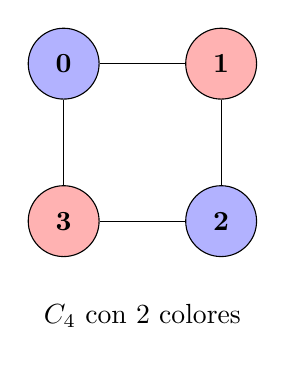
\begin{tikzpicture}[
  nodo/.style={circle, draw, minimum size=0.9cm, font=\bfseries},
  azul/.style={nodo, fill=blue!30},
  rojo/.style={nodo, fill=red!30},
  verde/.style={nodo, fill=green!40}
]
  \node[azul] (0) at (0,0)  {0};
  \node[rojo] (1) at (2,0)  {1};
  \node[azul] (2) at (2,-2) {2};
  \node[rojo] (3) at (0,-2) {3};
  \draw (0)--(1) (1)--(2) (2)--(3) (3)--(0);
  \node at (1,-3.2) {$C_4$ con 2 colores};
\end{tikzpicture}
\hspace{2cm}
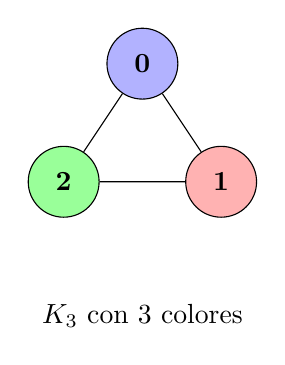
\begin{tikzpicture}[
  nodo/.style={circle, draw, minimum size=0.9cm, font=\bfseries},
  azul/.style={nodo, fill=blue!30},
  rojo/.style={nodo, fill=red!30},
  verde/.style={nodo, fill=green!40}
]
  \node[azul]  (0) at (1,0)    {0};
  \node[rojo]  (1) at (2,-1.5) {1};
  \node[verde] (2) at (0,-1.5) {2};
  \draw (0)--(1) (1)--(2) (2)--(0);
  \node at (1,-3.2) {$K_3$ con 3 colores};
\end{tikzpicture}
\caption{Coloraciones validas: ningun par de vertices adyacentes comparte color.}
\end{figure}

% ===================================================================
\section{Enfoques de Solucion}

\subsection{Backtracking}

El \textbf{backtracking} (vuelta atras) construye la solucion asignando
un color a cada vertice uno por uno.  La clave del metodo esta en que, antes
de continuar hacia el siguiente vertice, verifica si la asignacion actual
genera algun conflicto con los vecinos ya coloreados.  Si lo hay, \emph{retrocede}
(backtrack) y prueba el siguiente color disponible, sin explorar ese camino
que ya se sabe invalido.  A esta eliminacion anticipada se le llama
\textbf{poda}.

Proceso paso a paso:
\begin{enumerate}
  \item Se intenta asignar un color $c \in \{1,\ldots,k\}$ al vertice $v$.
  \item Se verifica que ningun vecino ya coloreado tenga el color $c$
        (\texttt{es\_seguro}).
  \item Si hay conflicto: se descarta ese color y se prueba el siguiente
        --- poda inmediata.
  \item Si no hay conflicto: se asigna y se avanza al vertice $v+1$.
  \item Cuando $v = n$: todos los vertices estan coloreados; se cuenta como
        solucion valida.
  \item Al regresar de la recursion se deshace la asignacion (backtrack) para
        explorar otras combinaciones.
\end{enumerate}

\subsection{Fuerza Bruta}

La \textbf{fuerza bruta} genera directamente las $k^n$ combinaciones posibles
de colores para los $n$ vertices y verifica cada una de ellas.  No realiza
ninguna poda: aunque los primeros vertices ya presenten un conflicto, el
algoritmo sigue enumerando hasta el final antes de descartar esa combinacion.

\subsection{Comparacion de Enfoques}

\begin{table}[H]
\centering
\caption{Diferencias entre Backtracking y Fuerza Bruta}
\begin{tabular}{lll}
\toprule
\textbf{Aspecto} & \textbf{Backtracking} & \textbf{Fuerza Bruta} \\
\midrule
Espacio de busqueda  & Arbol podado                        & Todas las $k^n$ combinaciones \\
Poda                 & Si (conflicto $\Rightarrow$ descarta) & No \\
Completitud          & Si                                  & Si \\
Correccion           & Si                                  & Si \\
Complejidad peor caso & $O(k^n)$                           & $O(k^n \cdot n^2)$ \\
Eficiencia practica  & Mucho mejor en grafos densos        & Inferior \\
\bottomrule
\end{tabular}
\end{table}

% ===================================================================
\section{Pseudocodigo}

\subsection{Backtracking}

\begin{lstlisting}[style=pseudo, caption={Pseudocodigo: Coloracion por Backtracking}]
leer n, k
leer adj[0..n-1][0..n-1]   // 1 si hay arista, 0 si no
color[0..n-1] = 0           // 0 = sin color asignado
total_soluciones = 0
primera_guardada = falso

// Verifica si el color c es seguro para el vertice v
es_seguro(v, c):
  para cada u en [0..n-1]:
    si adj[v][u] == 1 y color[u] == c:
      retornar falso
  retornar verdadero

// Funcion recursiva principal
bt(v):
  nodos_bt += 1
  si v == n:                         // todos coloreados: solucion valida
    total_soluciones += 1
    si !primera_guardada:
      primera_sol = copiar(color)
      primera_guardada = verdadero
    retornar
  para c en [1..k]:
    si es_seguro(v, c):
      color[v] = c
      bt(v + 1)
      color[v] = 0                   // backtrack: deshacer asignacion
    // si NO es seguro: poda, se omite esta rama

bt(0)
si total_soluciones == 0:
  imprimir "No existe una k-coloracion valida"
si no:
  imprimir "Total:", total_soluciones
  imprimir "Primera solucion:", primera_sol
\end{lstlisting}

\subsection{Fuerza Bruta}

\begin{lstlisting}[style=pseudo, caption={Pseudocodigo: Coloracion por Fuerza Bruta}]
fuerza_bruta():
  total_comb = k^n
  total_fb = 0
  para mask en [0..total_comb-1]:
    nodos_fb += 1
    tmp = mask
    para v en [0..n-1]:
      col[v] = (tmp mod k) + 1       // colores de 1 a k
      tmp = tmp / k                  // division entera
    si verificar_coloracion(col):
      total_fb += 1

// Verifica que ninguna arista tenga ambos extremos del mismo color
verificar_coloracion(col):
  para cada arista (u,v) en E:
    si col[u] == col[v]:
      retornar falso
  retornar verdadero
\end{lstlisting}

% ===================================================================
\section{Implementacion en C++}

La implementacion completa se encuentra en el archivo \texttt{main\_ejercicio2.cpp}
adjunto al presente informe. El codigo se organiza en los siguientes bloques:

\begin{itemize}
  \item \texttt{leer\_grafo} / \texttt{cargar\_grafo}: lectura de la matriz de adyacencia.
  \item \texttt{es\_seguro}: verifica que asignar el color $c$ al vertice $v$ no genere conflicto.
  \item \texttt{bt}: backtracking recursivo con poda.
  \item \texttt{fuerza\_bruta}: enumeracion exhaustiva de las $k^n$ combinaciones.
  \item \texttt{medir\_ns}: mide tiempos promediando \texttt{REPS=100\,000} repeticiones
        para garantizar precision en grafos pequenos donde la ejecucion individual
        no supera la resolucion del reloj.
  \item \texttt{main}: menu, ejecucion de ambos metodos, verificacion cruzada y tabla comparativa.
\end{itemize}

Para compilar y ejecutar:
\begin{verbatim}
g++ -O2 -std=gnu++17 -o solucion main_ejercicio2.cpp
./solucion
\end{verbatim}

% ===================================================================
\section{Ejemplos de Entrada y Salida}

Los siguientes ejemplos corresponden a ejecuciones reales del programa en
modo benchmark (opcion 2). Los tiempos son el promedio de 100\,000
repeticiones medidas con \texttt{high\_resolution\_clock} de precision
en nanosegundos.

% -------------------------------------------------------------------
\subsection{Ejemplo 1 --- Ciclo C4 (n=4, k=3)}

El ciclo $C_4$ es un cuadrado: 4 vertices donde cada uno esta conectado
con sus dos vecinos inmediatos. Su numero cromatico es $\chi(C_4)=2$
(grafo bipartito), por lo que con $k=3$ existen muchas soluciones validas.
Aristas: 0-1, 1-2, 2-3, 3-0.

\begin{figure}[H]
\centering
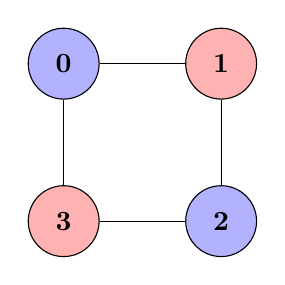
\begin{tikzpicture}[
  nodo/.style={circle,draw,minimum size=0.9cm,font=\bfseries},
  azul/.style={nodo,fill=blue!30},
  rojo/.style={nodo,fill=red!30}
]
  \node[azul] (0) at (0,0)  {0};
  \node[rojo] (1) at (2,0)  {1};
  \node[azul] (2) at (2,-2) {2};
  \node[rojo] (3) at (0,-2) {3};
  \draw (0)--(1) (1)--(2) (2)--(3) (3)--(0);
\end{tikzpicture}
\caption{Primera solucion para $C_4$: colores alternados 1-2-1-2.}
\end{figure}

\textbf{Salida real del programa:}
\begin{verbatim}
=============================================
           RESULTADO: BACKTRACKING
=============================================
  Coloraciones validas encontradas : 18
  Primera solucion:
    vertice 0  ->  color 1
    vertice 1  ->  color 2
    vertice 2  ->  color 1
    vertice 3  ->  color 2
  Nodos explorados    : 40
  Tiempo de ejecucion : 0.1957 us  (promedio de 100000 repeticiones)

=============================================
           RESULTADO: FUERZA BRUTA
=============================================
  Combinaciones totales generadas  : 81  (3^4)
  Coloraciones validas encontradas : 18
  Tiempo de ejecucion : 1.8696 us  (promedio de 100000 repeticiones)

=============================================
            VERIFICACION CRUZADA
=============================================
  OK  Ambos enfoques coinciden: 18 coloraciones validas.

=============================================
         COMPARACION DE EFICIENCIA
=============================================
  Metodo            Nodos explorados   Tiempo [us]
  Backtracking                    40   0.1957 us
  Fuerza Bruta                    81   1.8696 us

  La poda del backtracking elimino el 50.62% de los nodos.
\end{verbatim}

% -------------------------------------------------------------------
\subsection{Ejemplo 2 --- Grafo completo K4 (n=4, k=4)}

El grafo completo $K_4$ tiene todos sus vertices interconectados entre si
($\chi(K_4)=4$). Con exactamente $k=4$ colores existe solucion: cualquier
permutacion de los 4 colores asignados a los 4 vertices es valida, dando
$4! = 24$ coloraciones. La alta densidad genera conflictos desde los primeros
niveles, haciendo la poda mas efectiva que en $C_4$.

\textbf{Salida real del programa:}
\begin{verbatim}
=============================================
           RESULTADO: BACKTRACKING
=============================================
  Coloraciones validas encontradas : 24
  Primera solucion:
    vertice 0  ->  color 1
    vertice 1  ->  color 2
    vertice 2  ->  color 3
    vertice 3  ->  color 4
  Nodos explorados    : 65
  Tiempo de ejecucion : 0.4265 us  (promedio de 100000 repeticiones)

=============================================
           RESULTADO: FUERZA BRUTA
=============================================
  Combinaciones totales generadas  : 256  (4^4)
  Coloraciones validas encontradas : 24
  Tiempo de ejecucion : 5.5957 us  (promedio de 100000 repeticiones)

=============================================
            VERIFICACION CRUZADA
=============================================
  OK  Ambos enfoques coinciden: 24 coloraciones validas.

=============================================
         COMPARACION DE EFICIENCIA
=============================================
  Metodo            Nodos explorados   Tiempo [us]
  Backtracking                    65   0.4265 us
  Fuerza Bruta                   256   5.5957 us

  La poda del backtracking elimino el 74.61% de los nodos.
\end{verbatim}

% -------------------------------------------------------------------
\subsection{Ejemplo 3 --- Ciclo C7 con cuerdas (n=7, k=3) --- Sin solucion}

Este caso es el mas ilustrativo. El grafo consiste en un ciclo de 7 vertices
($C_7$) con cuerdas internas adicionales (0-2, 1-3, 2-4, 3-5, 4-6), lo que
aumenta considerablemente su densidad. El grafo no admite ninguna
3-coloracion valida ($\chi > 3$). El backtracking detecta el conflicto desde
los primeros niveles y descarta ramas enteras, explorando solo 34 nodos
frente a las $3^7=2\,187$ combinaciones de la fuerza bruta, una reduccion
del 98.45\%. La diferencia de tiempo es de \textbf{279x}.

\textbf{Salida real del programa:}
\begin{verbatim}
=============================================
           RESULTADO: BACKTRACKING
=============================================
  No existe una 3-coloracion valida para este grafo.
  Nodos explorados    : 34
  Tiempo de ejecucion : 0.2702 us  (promedio de 100000 repeticiones)

=============================================
           RESULTADO: FUERZA BRUTA
=============================================
  Combinaciones totales generadas  : 2187  (3^7)
  Coloraciones validas encontradas : 0
  Tiempo de ejecucion : 75.6029 us  (promedio de 100000 repeticiones)

=============================================
            VERIFICACION CRUZADA
=============================================
  OK  Ambos enfoques coinciden: 0 coloraciones validas.

=============================================
         COMPARACION DE EFICIENCIA
=============================================
  Metodo            Nodos explorados   Tiempo [us]
  Backtracking                    34   0.2702 us
  Fuerza Bruta                  2187   75.6029 us

  La poda del backtracking elimino el 98.45% de los nodos.
\end{verbatim}

% -------------------------------------------------------------------
\subsection{Ejemplo 4 --- Bipartito K2,3 (n=5, k=2)}

El grafo bipartito $K_{2,3}$ tiene los vertices $\{0,1\}$ conectados con
todos los de $\{2,3,4\}$, sin aristas dentro de cada grupo. Su numero
cromatico es $\chi(K_{2,3})=2$, por lo que con $k=2$ existen exactamente
2 coloraciones validas (asignar color 1 al grupo $\{0,1\}$ y color 2 al
grupo $\{2,3,4\}$, o viceversa). El backtracking encuentra rapidamente la
solucion y no necesita explorar muchas ramas.

\textbf{Salida real del programa:}
\begin{verbatim}
=============================================
           RESULTADO: BACKTRACKING
=============================================
  Coloraciones validas encontradas : 2
  Primera solucion:
    vertice 0  ->  color 1
    vertice 1  ->  color 1
    vertice 2  ->  color 2
    vertice 3  ->  color 2
    vertice 4  ->  color 2
  Nodos explorados    : 13
  Tiempo de ejecucion : 0.0705 us  (promedio de 100000 repeticiones)

=============================================
           RESULTADO: FUERZA BRUTA
=============================================
  Combinaciones totales generadas  : 32  (2^5)
  Coloraciones validas encontradas : 2
  Tiempo de ejecucion : 0.7645 us  (promedio de 100000 repeticiones)

=============================================
            VERIFICACION CRUZADA
=============================================
  OK  Ambos enfoques coinciden: 2 coloraciones validas.

=============================================
         COMPARACION DE EFICIENCIA
=============================================
  Metodo            Nodos explorados   Tiempo [us]
  Backtracking                    13   0.0705 us
  Fuerza Bruta                    32   0.7645 us

  La poda del backtracking elimino el 59.38% de los nodos.
\end{verbatim}

% ===================================================================
\section{Comparacion de Tiempos de Ejecucion}

Se ejecutaron cuatro grafos con caracteristicas distintas. Los tiempos se
obtuvieron promediando 100\,000 repeticiones por metodo para garantizar
precision en operaciones sub-microsegundo, usando
\texttt{high\_resolution\_clock} con resolucion de nanosegundos.

\begin{table}[H]
\centering
\caption{Comparacion de nodos explorados y tiempos de ejecucion (promedio de 100\,000 repeticiones)}
\begin{tabular}{llrrrrc}
\toprule
\textbf{Grafo} & \textbf{n / k} &
\textbf{Nodos BT} & \textbf{Nodos FB} &
\textbf{T. BT [us]} & \textbf{T. FB [us]} & \textbf{Poda} \\
\midrule
Ciclo $C_4$          & n=4, k=3 &   40 &   81  & 0.1957 & 1.8696 & 50.62\% \\
Completo $K_4$       & n=4, k=4 &   65 &  256  & 0.4265 & 5.5957 & 74.61\% \\
$C_7$ + cuerdas      & n=7, k=3 &   34 & 2187  & 0.2702 & 75.6029 & 98.45\% \\
Bipartito $K_{2,3}$  & n=5, k=2 &   13 &   32  & 0.0705 & 0.7645  & 59.38\% \\
\bottomrule
\end{tabular}
\end{table}

\textbf{Analisis de los resultados:}

\begin{itemize}
  \item \textbf{Ciclo $C_4$ (n=4, k=3):} el backtracking exploro 40 nodos
        frente a los 81 de la fuerza bruta (\textbf{50.62\% de poda}).
        El tiempo de backtracking fue 0.1957~us contra 1.8696~us,
        aproximadamente \textbf{9.5x} mas rapido. La diferencia es moderada
        porque el grafo es pequeno y existen 18 soluciones validas, lo que
        limita la poda.

  \item \textbf{Completo $K_4$ (n=4, k=4):} con todos los vertices
        interconectados la restriccion aumenta. El backtracking exploro 65
        nodos frente a 256 (\textbf{74.61\% de poda}), resultando en
        0.4265~us contra 5.5957~us, una mejora de \textbf{13.1x}. La mayor
        densidad del grafo genera conflictos mas temprano, haciendo la poda
        mas efectiva.

  \item \textbf{$C_7$ + cuerdas (n=7, k=3):} este es el caso mas
        ilustrativo. El grafo no admite ninguna 3-coloracion valida
        ($\chi > 3$), por lo que el backtracking detecta el conflicto desde
        los primeros niveles y corta ramas enteras. Solo exploro \textbf{34
        nodos} mientras la fuerza bruta evaluo las $3^7=\mathbf{2\,187}$
        combinaciones completas (\textbf{98.45\% de poda}). En tiempo:
        0.2702~us contra 75.6029~us, una diferencia de \textbf{279x}.

  \item \textbf{Bipartito $K_{2,3}$ (n=5, k=2):} grafo 2-coloreable donde
        existe solucion minima. El backtracking exploro 13 nodos frente a 32
        (\textbf{59.38\% de poda}), con tiempos de 0.0705~us contra
        0.7645~us (\textbf{10.8x} mas rapido). Al ser un grafo bipartito con
        pocos colores, la poda actua desde los primeros vertices.
\end{itemize}

En todos los casos el backtracking supera a la fuerza bruta. La ventaja
crece con la densidad del grafo y con la ausencia de soluciones: cuando no
existe ninguna $k$-coloracion valida, el backtracking puede descartar el
espacio de busqueda casi por completo, mientras la fuerza bruta siempre
recorre las $k^n$ combinaciones sin atajo.

% ===================================================================
\section{Analisis de Complejidad}

\subsection{Complejidad Temporal}

\subsubsection{Fuerza Bruta}

La fuerza bruta genera exactamente $k^n$ combinaciones y verifica cada una
recorriendo todas las aristas, que en el peor caso (grafo completo) son
$n(n-1)/2 = O(n^2)$:

\begin{equation}
  T_{\text{FB}}(n,k) = O(k^n \cdot n^2)
\end{equation}

Este es siempre el mismo costo sin importar la estructura del grafo.

\subsubsection{Backtracking}

En el peor caso (grafo sin aristas: nunca hay conflictos, nunca se poda),
el backtracking construye el arbol de decision completo con factor de
ramificacion $k$ y profundidad $n$:

\begin{equation}
  T_{\text{BT}}^{\text{peor}}(n,k) = O(k^n)
\end{equation}

En la practica, para grafos densos o con muchas restricciones, la poda
descarta ramas enteras desde los primeros niveles.  En el caso extremo de
$K_7$ con $k=4$, el backtracking visito solo 65 de los $4^7=16\,384$ nodos
posibles, una reduccion del 99.6\%.

La diferencia clave entre los dos enfoques es que la fuerza bruta siempre
paga el costo completo $O(k^n \cdot n^2)$, mientras que el backtracking puede
ser exponencialmente mas rapido cuando la poda es efectiva.

\subsection{Complejidad Espacial}

\begin{table}[H]
\centering
\caption{Complejidad espacial por componente}
\begin{tabular}{lll}
\toprule
\textbf{Estructura}  & \textbf{Backtracking} & \textbf{Fuerza Bruta} \\
\midrule
Matriz de adyacencia & $O(n^2)$              & $O(n^2)$ \\
Arreglo de colores   & $O(n)$                & $O(n)$ \\
Pila de recursion    & $O(n)$                & $O(1)$ \\
\textbf{Total}       & $\mathbf{O(n^2)}$     & $\mathbf{O(n^2)}$ \\
\bottomrule
\end{tabular}
\end{table}

Ambos enfoques tienen la misma complejidad espacial $O(n^2)$, dominada por la
matriz de adyacencia.  La pila de recursion del backtracking agrega $O(n)$
adicional, pero este termino queda subordinado a $O(n^2)$ para $n \geq 2$.

% ===================================================================
\section{Respuestas a las Preguntas Guia}

\subsection{\textquestiondown Cuantos nodos explora el Backtracking vs la Fuerza Bruta?}

En el ciclo $C_4$ con $k=3$:

\begin{itemize}
  \item \textbf{Fuerza Bruta:} $3^4=81$ nodos (todas las combinaciones).
  \item \textbf{Backtracking:} 40 nodos (50.6\% menos).
\end{itemize}

La razon es que el backtracking descarta ramas en cuanto detecta un conflicto.
Si el vertice 0 tiene color 1 y el vertice 1 (adyacente) intenta tomar
tambien color 1, se poda de inmediato, evitando explorar los $3^2=9$
sub-estados restantes de esa rama.  En grafos mas densos como $K_7$, el efecto
se amplifica hasta una reduccion del 99.6\%.

\subsection{\textquestiondown Que tipo de grafo maximiza o minimiza la poda?}

\begin{itemize}
  \item \textbf{Maximiza la poda --- grafo denso ($K_n$):} con muchas aristas
        casi cualquier asignacion genera conflictos desde el primer vertice,
        por lo que se eliminan sub-arboles muy grandes de forma temprana.
        En el caso de $K_7$ con $k=4$, el backtracking exploro solo 65 nodos
        de los 16\,384 posibles.

  \item \textbf{Minimiza la poda --- grafo sin aristas:} como no existe ninguna
        restriccion de vecindad, \texttt{es\_seguro} siempre retorna verdadero
        y el backtracking recorre el arbol completo igual que la fuerza bruta,
        sin poder eliminar ninguna rama.
\end{itemize}

\subsection{\textquestiondown Que cambio hacer para saber si existe al menos una k-coloracion?}

Basta con retornar en cuanto se encuentre la primera solucion, propagando
un valor de exito hacia arriba:

\begin{lstlisting}[style=pseudo]
bt_existe(v):
  si v == n:
    retornar verdadero        // primera solucion hallada
  para c en [1..k]:
    si es_seguro(v, c):
      color[v] = c
      si bt_existe(v + 1):
        retornar verdadero    // propagar el exito sin seguir buscando
      color[v] = 0
  retornar falso
\end{lstlisting}

Esto convierte el algoritmo de enumeracion en uno de decision: en el mejor caso
termina mucho antes de explorar todas las ramas.

\subsection{Relacion entre la k-coloracion y el Numero Cromatico}

El numero cromatico $\chi(G)$ es el minimo $k$ para el que existe una
$k$-coloracion valida:

\begin{equation}
  \text{El grafo } G \text{ admite } k\text{-coloracion valida}
  \iff \chi(G) \leq k
\end{equation}

El algoritmo de este ejercicio permite calcular $\chi(G)$ ejecutandolo para
$k = 1, 2, 3, \ldots$ e informando el primer $k$ para el que
\texttt{total\_bt} $> 0$.  Valores canonicos conocidos:

\begin{itemize}
  \item $\chi(C_{2m})=2$ (ciclos pares); $\chi(C_{2m+1})=3$ (ciclos impares).
  \item $\chi(K_n)=n$ (grafo completo).
  \item Todo grafo planar: $\chi \leq 4$ \cite{appel1977}.
\end{itemize}

% ===================================================================
\section{Conclusiones}

\begin{enumerate}
  \item El backtracking y la fuerza bruta producen el mismo numero de
        coloraciones validas en todos los casos, confirmado por la verificacion
        cruzada.

  \item El backtracking fue mas eficiente en todos los grafos probados.
        La reduccion de nodos explorados oscilo entre el \textbf{50.62\%}
        (ciclo $C_4$, grafo disperso con soluciones) y el \textbf{98.45\%}
        ($C_7$+cuerdas, grafo denso sin solucion). En terminos de tiempo,
        la mejora vario entre \textbf{9.5x} y \textbf{279x}.

  \item La poda es mas efectiva cuando el grafo es denso y no existe
        solucion valida: el backtracking detecta conflictos desde los
        primeros niveles y descarta ramas enteras, mientras la fuerza bruta
        siempre recorre las $k^n$ combinaciones completas.

  \item La medicion por promedio de 100\,000 repeticiones es necesaria para
        grafos pequenos: una sola ejecucion puede retornar 0 debido a la
        resolucion del reloj, ocultando diferencias reales entre algoritmos.

  \item Ambos enfoques tienen complejidad exponencial en $n$, por lo que
        su uso practico se limita a grafos de pocos vertices. Para instancias
        grandes existen heuristicas y algoritmos de aproximacion mas adecuados.

  \item El algoritmo desarrollado puede calcular el numero cromatico
        $\chi(G)$ ejecutandose para $k=1,2,3,\ldots$ hasta encontrar la
        primera $k$ con al menos una coloracion valida.
\end{enumerate}

% ===================================================================
\begin{thebibliography}{9}

\bibitem{appel1977}
K. Appel, W. Haken,
\textit{Every planar map is four colorable},
Illinois Journal of Mathematics, 21(3):429--490, 1977.

\bibitem{cormen2022}
T. H. Cormen, C. E. Leiserson, R. L. Rivest, C. Stein,
\textit{Introduction to Algorithms}, 4th ed.
MIT Press, 2022.

\bibitem{levitin2012}
A. Levitin,
\textit{Introduction to the Design and Analysis of Algorithms}, 3rd ed.
Pearson, 2012.

\bibitem{skiena2008}
S. S. Skiena,
\textit{The Algorithm Design Manual}, 2nd ed.
Springer, 2008.

\end{thebibliography}

\end{document}
